\documentclass[a4paper]{article}

\usepackage[english]{babel}
\usepackage[utf8]{inputenc}
\usepackage{amsmath}
\usepackage{amssymb}
\usepackage{graphicx}
\usepackage[colorinlistoftodos]{todonotes}
\usepackage[margin=0.7in]{geometry}
\usepackage[numbers]{natbib}




\newcommand{\argmin}{\operatornamewithlimits{arg\ min}}

\usepackage{pgfplots}
\pgfplotsset{compat=1.10}
%\newcommand\gauss[2]{1/(#2*sqrt(2*pi))*exp(-((x-#1)^2)/(2*#2^2))}

%%This is all the fragment needed to use the URW Palladio Font
%\usepackage[sc]{mathpazo}
%\linespread{1.05}         % Palladio needs more leading (space between lines)
%\usepackage[T1]{fontenc}
%% End of fragment

\title{Math for Machine Learning}

\author{Author: Parameswaran Raman}

\date{\today}

\begin{document}

\pgfmathdeclarefunction{gauss}{3}{%
  \pgfmathparse{1/(#3*sqrt(2*pi))*exp(-((#1-#2)^2)/(2*#3^2))}%
}

\maketitle

\begin{abstract}
\noindent In this post, I want to discuss some of the pre-requisites for Machine Learning (citing specific examples where they come up). I have given very high-level explanations below and cut corners at several places as I do not want to get into the depth. My intention here is not to explain any concept precisely, but to merely lay down enough of them on the table to emphasize the role of Mathematics.
\end{abstract}

\section{So, why so much Math?}

\noindent Machine Learning is an incredibly modern field that borrows heavily from several areas of Mathematics. Having evolved as an inter-disciplinary field which is very applied (driven by data), it has captured concepts, intuition and theory from several places. Being at such an intersection of diverse areas of mathematics and computer science is what makes research in Machine Learning so exciting and challenging! \\

\noindent At this point, I would like to mention {\it Physics} as an analogy. I consider Machine Learning to be very similar to Physics as a discipline, primarily because both are applied areas by nature governed by deep mathematical foundations. It turns out, much of the pre-requisite Math for Machine Learning (Multi-variable calculus, linear algebra) applies to Physics too. Another similarity between the two fields is their philosophy and connection to the real world. In both cases, we try to model the real world phenomena by coming up with hypothesis and backing it up with experiments. This in turn leads us to a better understanding of the black-box that generates events in the real world (or data in case of machine learning). \\

\noindent \textit{"Imagine being in a battlefield without knowing how to use the weapons you have, (or worse still, not having the weapons at all)!"} \\

\noindent That's exactly how it feels when you set out to do research in machine learning without knowing enough about the fundamental areas underlying it. Without the right intuition, it becomes very hard to build new algorithms or extend existing ones.\\

\noindent Below are the key useful areas:

\subsection{Algorithms \& Complexity}
\textit{Knowledge of basic data structures such as arrays/trees/hash tables, programming techniques like dynammic programming, graphs, space and time complexity requirements for a given method, randomized algorithms, sublinear algorithms}.\\ \\
How do you convince someone that your learning algorithm is more space and/or time efficient (and hence scalable) on big datasets? Exploiting sparsity in the data sets might lead you to better performing algorithms; but how do you qualitatively compare their performance? With data getting more and more massive, going through it entirely is not feasible and therefore sometimes even linear time algorithms maybe too slow. This has led to the field of sub-linear algorithms which work by inspecting only a tiny fraction of the entire data. Property Testing is a closely related topic where the algorithm queries about some property of the input with a time complexity much smaller than the size of the input. These are relatively modern areas in theoretical computer science which have a direct impact on machine learning. Randomized algorithms is another highly useful field that has helped solve several big data problems, for eg large matrix problems have been very successfully dealt with using randomization techniques.\\

\subsection{Linear Algebra}
\textit{Rank of a Matrix, Matrix Vector products, Column Spaces and Null Spaces of a matrix, Eigen Values and Vectors, SVD factorization of a matrix, positive-definiteness of a matrix}. \\ \\
Linear Algebra plays a super heavy role in understanding Optimization methods used for Machine Learning. Many problems in machine learning can be expressed as a simple {\it least-squares} optimization problem. What is interesting is every least-squares problem can be turned into a Quadratic Program (ie, an optimization problem involving quadratic function of the variables). This is illustrated below:

\begin{equation} \label{eq:0}
\begin{split}
f(x) & = \frac{1}{2} \left\lVert \mathbf{Q} \boldsymbol{x} - \boldsymbol{c} \right\lVert ^2 \\
& = \frac{1}{2} (\mathbf{Q} \boldsymbol{x} - \boldsymbol{c})^T  (\mathbf{Q} \boldsymbol{x} - \boldsymbol{c}) \\
& = \frac{1}{2} (\boldsymbol{x}^T \mathbf{Q}^T \mathbf{Q} \boldsymbol{x} - \boldsymbol{x}^T \mathbf{Q}^T \boldsymbol{c} - \boldsymbol{c}^T \mathbf{Q} \boldsymbol{x} + \boldsymbol{c}^T \boldsymbol{c})
\end{split}
\end{equation}

\noindent Since $\boldsymbol{c}^T \boldsymbol{c}$ is a fixed quantity (constant), it is sufficient to solve the Quadratic Programming problem:
\begin{equation} \label{eq:0a}
\begin{split}
f(x) & = \frac{1}{2} \boldsymbol{x}^T \mathbf{A} \boldsymbol{x} + \boldsymbol{q}^T \boldsymbol{x} \\
\end{split}
\end{equation}, where $\mathbf{A} = \mathbf{Q}^T \mathbf{Q}$ and $\boldsymbol{q} = - \mathbf{Q}^T \boldsymbol{c}$. Observe that eqn(\ref{eq:0a}) has a matrix $\mathbf{A}$ in its first term. This matrix $\mathbf{A}$ is the {\it Hessian} (generalization of second-order derivatives to higher dimensions) and when it is positive-definite, the quadratic problem takes shape of a "bowl" in higher dimensions as shown below in Figure \ref{fig:BowlFunction}.

\begin{figure}[!htb]\label{fig:BowlFunction}
  \centering
  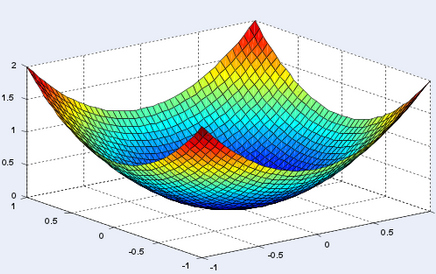
\includegraphics[width=0.5\columnwidth]{Convex_Function}\\
  \caption{Three dimensional "bowl" shaped function.}\label{fig:BowlFunction}
\end{figure}
\noindent As a consequence, it clearly has only one "unique" minima (global optimal solution). This concept is termed as "Convexity" (which is considered a {\it blessing for optimization} as such functions are well-understood and have some very attractive properties). Some of what I mentioned above constitute the nuts and bolts of Convex Optimization. Like-wise, when the matrix $\mathbf{A}$ is negative-definite, the function takes the shape of an inverted bowl and is not convex (therefore, has no global and unique minimum, but has a global maximum). Finally, when matrix $\mathbf{A}$ is indefinite, then the function takes a wierd form as below in Figure \ref{fig:SaddlePointFunction}.
\begin{figure}[!htb]\label{fig:SaddlePointFunction}
  \centering
  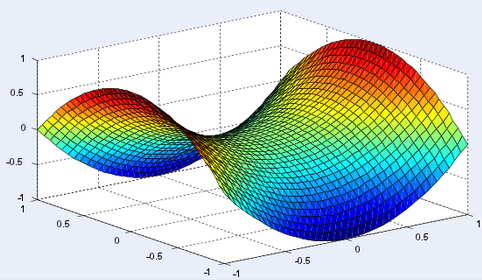
\includegraphics[width=0.5\columnwidth]{SaddlePoint_Function}\\
  \caption{Three dimensional function representing the saddle point problem.}\label{fig:SaddlePointFunction}
\end{figure}
As we can imagine, there is neither a global maximum or global minimum here. The surface infact looks like a "saddle" and for that reason called a saddle point.


Often although the data we obtain in the real world has very large dimensions (hundreds of thousands for example), it can often be reduced to a handful of useful dimensions that we can work with. This is called dimensionality reduction and uses ideas like low-rank approximation (rank of a data matrix determines the true dimensions of your data or how diverse your data can really be). Matrix Factorization methods are based on this and typical recommender systems like the one Netflix uses to predict movie ratings of a user, make use of it. Low-rank approximations are also used in other areas like Computer Vision and Information Retrieval as a tool for extracting correlations in data and removing noise from matrix-structured data. Algorithms in machine learning involve dozens of vector-vector multiplications (dot-products) and matrix-vector, matrix-matrix multiplications. All of these operations can be extremely costly and a bottleneck when trying to scale to big data. However, if we can cleverly manipulate or take advantage of special matrices which contains lots of zeros ("sparsity"), we can reduce such computations significantly. Eigen Vectors of a matrix come in handy in such situations.\\

\subsection{Probability Theory \& Statistics}
\begin{itemize}
\item Probability Theory: \textit{Counting and Combinatorial methods, Bayes' Theorem, Random Variables, Expection, Variance, Conditional and Joint Distributions, Moment Generating Functions, Exponential Family of Distributions}
\item Statistics: \textit{Maximum Likelihood Estimation, MAP, Prior and Posterior, Sampling methods, Gibbs}
\end{itemize}
As you would expect, this is the single-most important field which also conveys the essence of machine learning, namely - estimating the parameters of the data-generating process. Several machine learning methods have probabilistic interpretations and its common to hear the words {\it frequentist} and {\it bayesian} ways of doing things. One way to look at the difference between them is that the frequentist methods are concerned with estimating the parameters of their model that have the highest chance of generating the "current data"; this is called the Maximum Likelihood Estimation (MLE) and written as: \\

\begin{equation} \label{eq:1}
\begin{aligned}
&& \underset{\theta}{\operatorname{argmax}} \log {\cal L } (\theta) = \underset{\theta}{\operatorname{argmax}} \log P(Data|Parameters)
\end{aligned}
\end{equation}


\noindent  MLE has the tendency to overfit (generalize poorly on unseen data) and hence the Bayesian approach proposes incorporating historical evidence (based on "past data") into the current model. This is called the prior. The task of estimation then boils down to using Bayes' rule as below: \\

\begin{equation} \label{eq:2}
\begin{aligned}
& & P (Parameters|Data) = \frac{ P(Data|Parameters) P(Parameters)}{P(Data)}
\end{aligned}
\end{equation}

\noindent This can be equivalently written as : \\
\begin{equation} \label{eq:3}
\begin{aligned}
& & Posterior = \frac{ Likelihood \times Prior}{Normalizing Constant}
\end{aligned}
\end{equation}

\noindent Posterior gives us a probability distribution over the parameters and this is used in various ways to make predictions on the new data. As is evident by now, random variables play a huge part in estimation and we often deal with independence assumptions between them, work with their expected values and variances. It is also important to know the functional forms of some key probability distributions, for instance the most popularly used {\it Gaussian Distribution} (or normal distribution) $\sim \mathcal{N} (\mu, \sigma^2)$, which (in its univariate form) can be expressed as: \\

\begin{equation} \label{eq:4}
\begin{aligned}
& & \frac{1}{\sigma \sqrt{2 \pi}} \exp \left\{ - \frac{(x-\mu)^2}{2 \sigma^2} \right\}
\end{aligned}
\end{equation}

\noindent Methods of Sampling play an important role in optimization algorithms. Often the gradient (generalization of the derivative - this has been described in a bit more detail further down below) needs to be calculated over the entire data set and this is very expensive to compute in every iteration. To avoid this, algorithms like Stochastic Gradient Descent (SGD) randomly sample a data point and update its gradient alone, this makes the algorithm independent of the number of data points which means it will scale well. But, now we only selected specific data points; so our method becomes a bit biased. How can we make sure randomly selecting one point in each iteration will in the long run mimic the same behavior that we would have got if we had selected all the data points and computed the exact gradient? This is where techniques of designing unbiased sampling mechanisms come up. \\

\subsection{Multi-variable Calculus (Matrix-Vector Calculus)}
\textit{Vector-valued functions, Partial-Derivatives, Gradient, Directional Gradient, Hessian, Jacobian, Laplacian, Lagrange Multipliers} \\ \\
We know from our high-school calculus that in order to minimize or maximize a function you set its derivative to zero. Such a way of obtaining the solution is called the "closed-form" solution and this was an easy thing to do because back then, our functions then involved just handful of dimensions (often just a single variable). However, in machine learning its very common to deal with functions that operate on variables having hundreds of dimensions. What does derivative or slope even mean in such situations? That's where partial-derivatives come into the picture. You can look at them as derivatives of the function in each dimension of the variable. Combine these partial-derivatives into a vector and that gives us what is called the "Gradient". Similarly, taking the second-order derivative of Gradient gives us a matrix termed as the "Hessian". Also, in reality it is often not possible to obtain a "closed-form" solution (by setting the gradient to zero) because the dimensions of the gradient could be extremely high and storage/time required for this might be expensive. In such cases, knowledge of gradients and hessians help us define things like directions of descent and rate of descent which tell us how should we travel in our function space in order to get to the bottom most point (which represents the optimal solution). Thus at this point, we work using more abstract objects - "Vectors" and "Matrices" and should be reasonably comfortable with applying differential and integral calculus on them. This is also called "Vectorizing the equations", which Prof. Andrew Ng discusses in detail in one of his ML lectures (Refer Coursera). Below is an example of a simple objective function (linear regression with weights $x$, $N$ data points and $D$ dimensions) both in the vectorized and expanded notation. \\

Expanded notation:
\begin{equation} \label{eq:4}
\begin{aligned}
& & J(w) = \frac{1}{2} \sum_{i=1}^{N} (\sum_{j=1}^{D} a_{ij} x_j - b_i)^2
\end{aligned}
\end{equation}

Vectorized notation:
\begin{equation} \label{eq:5}
\begin{aligned}
& & J(w) = \frac{1}{2} \left\lVert \mathbf{A} \boldsymbol{x} - \boldsymbol{b} \right\rVert ^2
\end{aligned}
\end{equation}

\noindent As you can see the vectorized notation is not only compact and gets rid of the annoying summations but also is more expressive and makes us think more abstractly in terms of higher level objects like vectors (x and b) and matrices (A). Such representations also help us leverage all the rich properties that vectors and matrices provide us (that speed up our computation and make things easily parallelizable, to mention a few). What this also means is that, we need to now get comfortable with doing arithmetic in this new space. For instance, while moving terms around, we cannot divide by a matrix and instead have to compute the inverse (At this point, I should also mention that computing inverses of big matrices are expensive too and there are workarounds and techniques to deal with this). The method of Lagrangian multipliers is a standard way in calculus to maximize or minimize functions when there are constraints involved. This comes up a lot in Optimization. \\

\subsection{Real Analysis}
\textit{Properties of Sets and Sequences, Convergence of Sequence, Cauchy Sequences, Concepts from Topology like Open and Closed Sets, Metric Spaces, Limits and Continuity of functions, Differentiability} \\ \\
While this is the most rigorous of all mathematical fields I have mentioned, its importance is highly understated. For a person in Machine Learning, (quoting a friend of mine in his exact words) Real Analysis is a long-term investment. It gives you sufficient practice with the art of writing mathematics proofs in a rigorous manner and making precise statements without gaps and holes in your arguments. This is an extremely useful skill to acquire that helps you when writing and reading research papers. Although intuition and pictures are often good ways to describe and understand ideas; compressing them in a clear mathematical way is sometimes valuable as it avoids ambiguity. Analysis also helps one navigate more comfortably through some fundamental concepts in numerical optimization such as - sequences, what does it mean for a sequence to converge to a limit point, how do you define the rate of convergence, what does it mean for a sequence or set to have a \textit{sup} and \textit{inf}? While fields of Linear Algebra and Multi-variate calculus help you design optimization methods for machine learning, tools from Real Analysis will help you defend them and verify their correctness theoretically. \\

\subsection{Information Theory}
\textit{Entropy, Mutual Information, Information Gain, KL Divergence} \\ \\
This branch of applied mathematics deals with studying how to quantify information. Entropy for example quantifies the uncertainty involved in predicting the value of a random variable and intersects with other fields like Proability Theory. KL-Divergence is a widely used metric to measure how different two probability distributions are. \\

\noindent For the sake of completeness, let me mention that there are few other areas such as {\it Differential Geometry} and {\it Measure Theory} which make cameo appearances once in a while, but the show is predominently run by the ones above!

%\bibliographystyle{plainnat}
%\bibliography{refs.bib}
\end{document}